\chapter{Methodology}\label{chp:methodology}
In this chapter we explain the research methods used and rationalize their choice. Further, we present the pre processing and label selection, the detailed architecture of the networks and the different experiments that have been conducted. 
\section{Data}

As explained in Section~\ref{sec:coring}, the data has been gathered through coring and labelled by geologists. Further on, we will consider the geologists labels as the ground truth. We have gathered 1907 labeled images. 

\subsection{Label Selection}
 The labels of every image can be divided into different classes, see Figure~\ref{fig:classes}. For example, the class Lithology contains 10 different labels, each representing one of the possible lithologies. Not all images have labels in every classes, that is why some classes are under-represented. The classes Dominant Grain type, Diagenesis, Cutting description and Sorting have less than 1000 data points. This is not enough to produce good prediction, that is why we chose not to use them.
 
 For the classes that are sufficiently populated, we plot the distribution of the data points within those classes. On Figure~\ref{fig:litandstruct}, we can see the labels distribution for Lithology and Structures. The labels are extremely unbalanced, so trying to predict any other label than Lit1 for Lithology and Structure 1 or 2 for Structures would be very difficult. This is why we will not try to predict on those class. 
 The remaining classes : Porosity, Components, Dunham and DRT, have a good distribution of points within the class. They also give a good overview of the rock properties. If we are able to predict correctly on them, we will have an idea of how good the reservoir rock is. 
\begin{figure}
\begin{subfigure}{.5\textwidth}
  \centering
  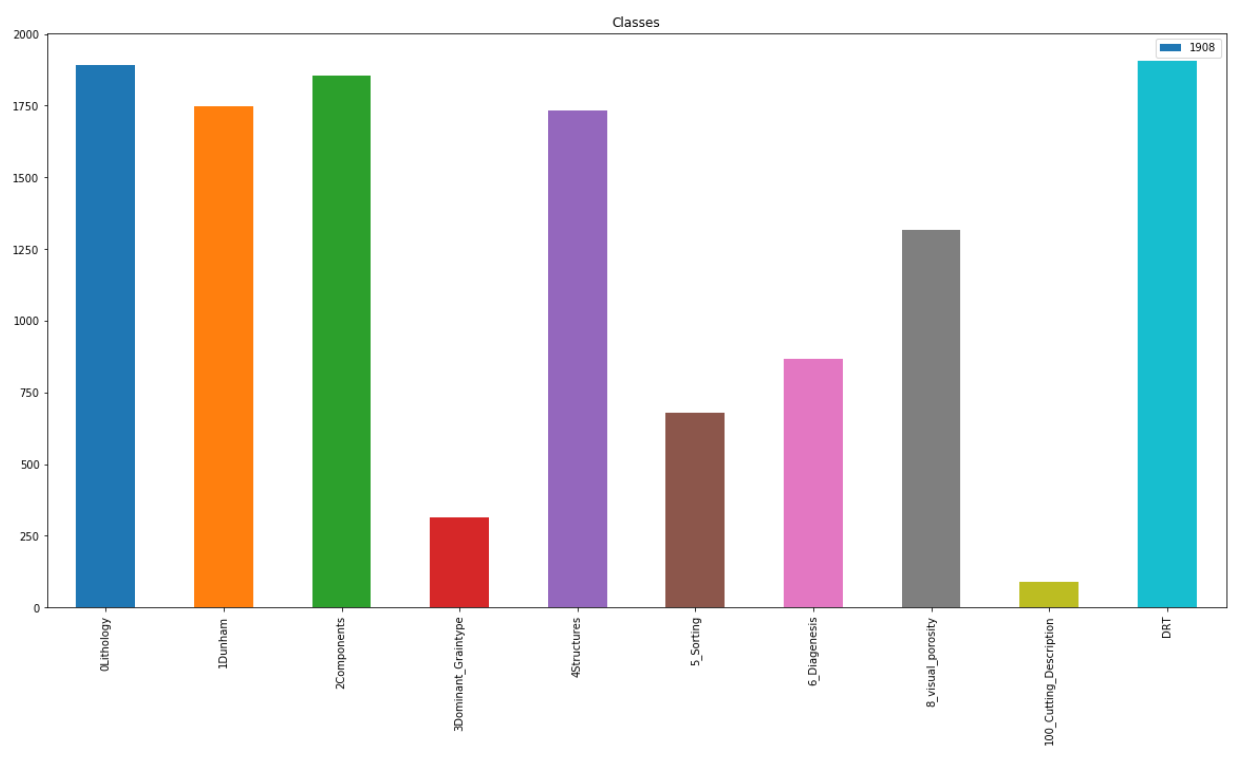
\includegraphics[width=.8\linewidth]{figures/03-classes.png}
  \caption{Classes over the samples}
  \label{fig:classes}
\end{subfigure}%
\begin{subfigure}{.5\textwidth}
  \centering
  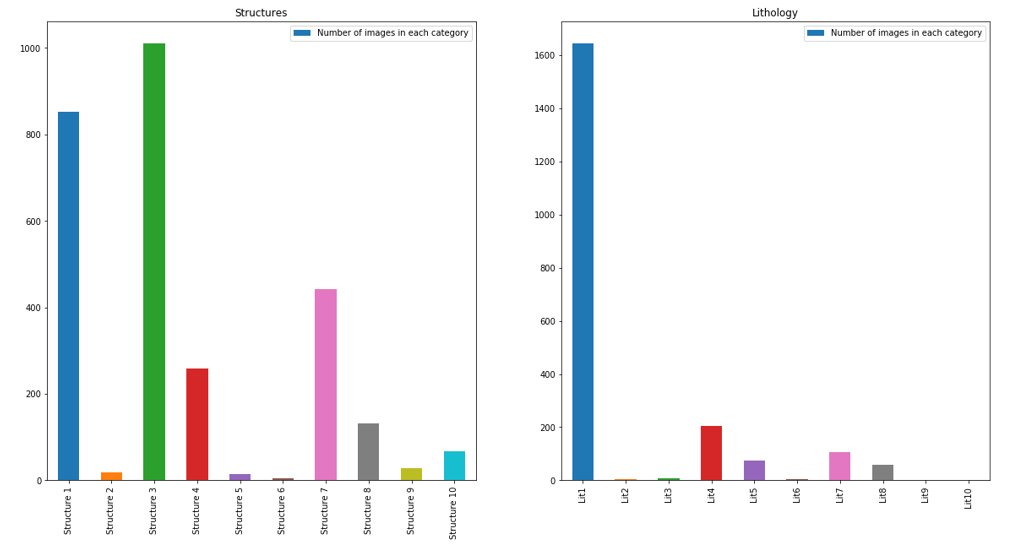
\includegraphics[width=.8\linewidth]{figures/03-boob.PNG}
  \caption{Lithology and Structure over samples}
  \label{fig:litandstruct}
\end{subfigure}
\caption[Classes distributions]{Distribution of different classes over the whole data set.}
\end{figure}


\subsection{Label pre-processing}
Once we selected the four labels to predict on, we looked into the details of the distribution and adapted it to make it easier to predict on. For the Dunham labels, the first class was under represented, only seven samples. So we decided to simply cut it out. We now have six classes that are almost homogeneously distributed, see Figure~\ref{fig:dunham}. 

For the porosity labels, there are two different levels of description of the porosity. The first level is the amount of porosity: no, minor, intermediate or abundant. The second is the kind of porosity: patchy or micro-porosity. In a first pass, we will only focus on the quantitative aspect: how much porosity do we observe in each sample, see Figure~\ref{fig:porolab}. A further analysis would be to determine what kind of porosity accounts for this total porosity. It might be considered at a later stage. Also, for this first experiment, after we have extracted four labels, we sorted them from no to abundant porosity. 

As shown on Figure~\ref{fig:drtlab} and Figure~\ref{fig:compolab}, the DRT and components class have a lot of different labels: 19 and 13 respectively. Some of them are not populated enough to be considered. Some of the labels we chose to keep are still under-represented but we believe they are populated enough to be predicted.

We can divide the classes into two main categories. The DRT and Dunham labels are single-label multi-class labels. It means that each image can only have one label within a class. The Components label are multi-labels multi-class labels, meaning that one image can have one or more label. The porosity has two levels of labels, so we can consider porosity as being both single-label (if we only look at the amount) or multi-label labels. 


As we can see on Figures~\ref{fig:dunhamlab} to ~\ref{fig:compolab}, our labels are not equally distributed. Thus, the network will be biased towards the most populated labels. A way to counter this would be to get more samples of the under represented class. But when one is trying to characterize a certain geographical area, it is normal to find rocks and components that are more present than others. We deal with this issue by calculating the loss with weights. We want to teach our model to give a higher weight to a sample with an under represented label, than one with a more represented label . This way, it should not favor most populated class. 

For single label classification, we calculate the weights of each class as follows: weight of class A is the total number of samples divided by the number of samples in class A.

For multi-label classification, the labels are represented as one-hot encoded vectors as we saw in section~\ref{sec:loss}. We calculate the weights as follows: weight of class A is the number of 0 in class A divided by the number of 1 in class A.

\begin{figure}
\begin{subfigure}{.5\textwidth}
  \centering
  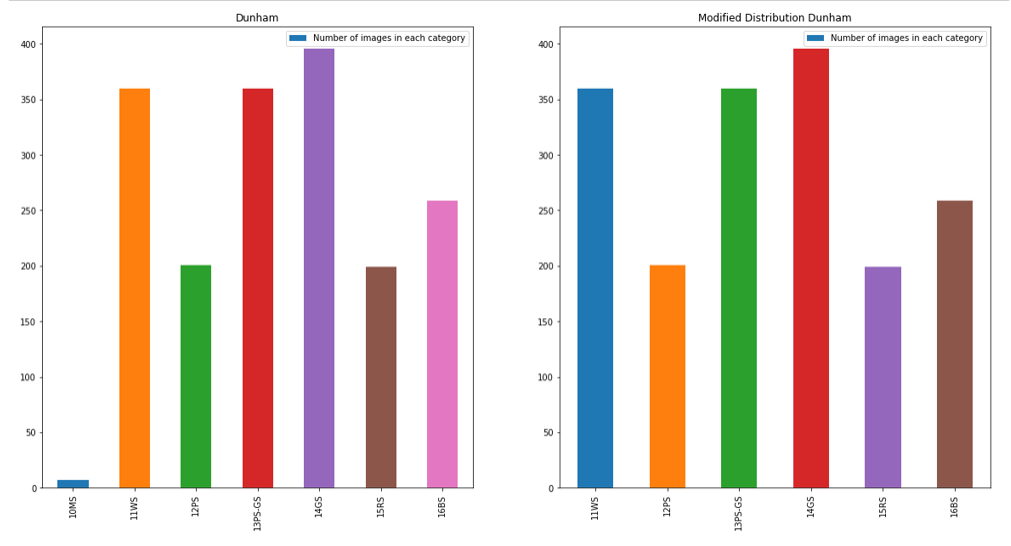
\includegraphics[width=.8\linewidth]{figures/03-Dunham.PNG}
  \caption{Dunham Labels}
  \label{fig:dunhamlab}
\end{subfigure}%
\begin{subfigure}{.5\textwidth}
  \centering
  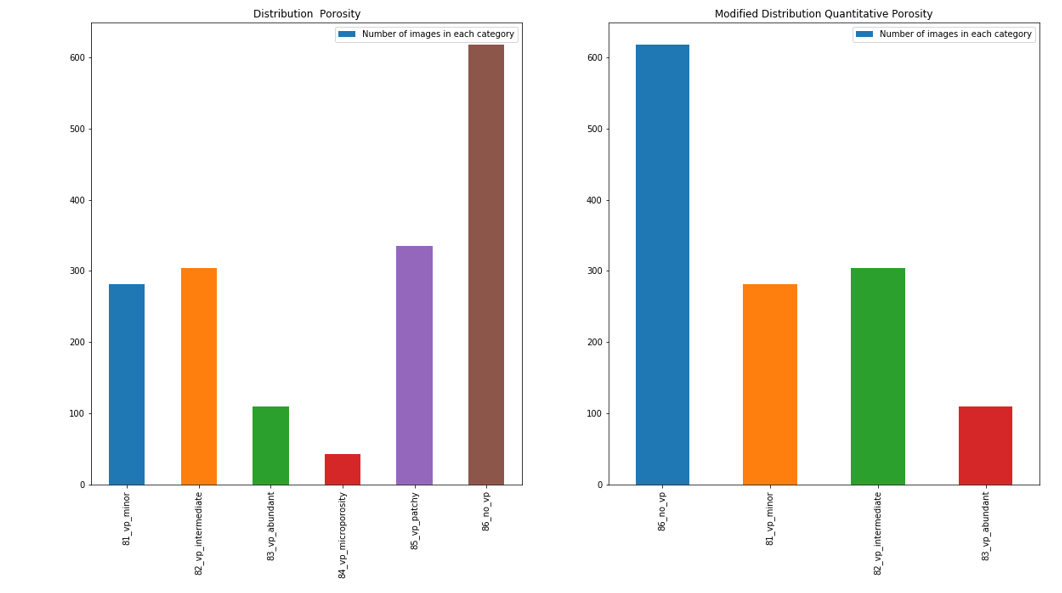
\includegraphics[width=.8\linewidth]{figures/03-porosity_baby.PNG}
  \caption{Porosity Labels}
  \label{fig:porolab}
\end{subfigure}
\begin{subfigure}{.5\textwidth}
  \centering
  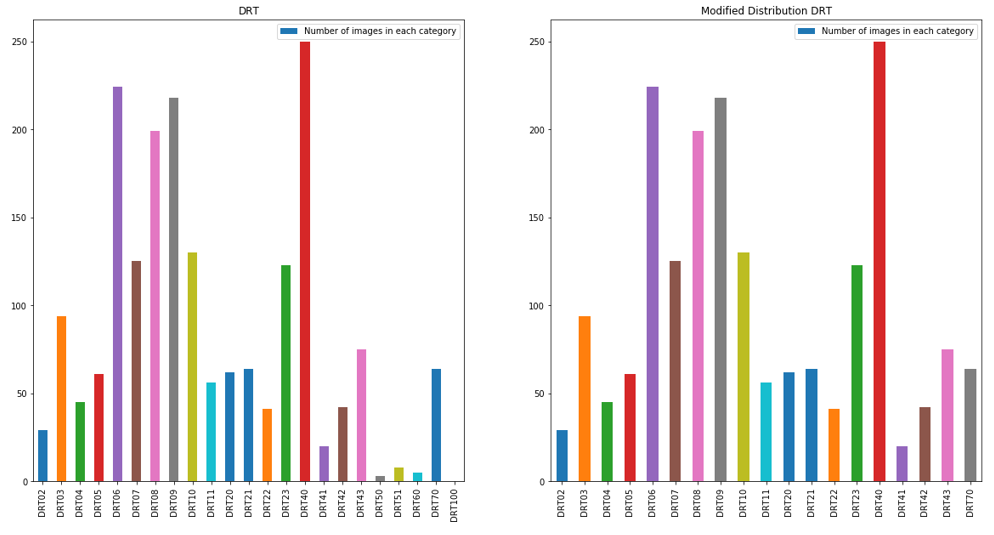
\includegraphics[width=.8\linewidth]{figures/03-DRT.PNG}
  \caption{DRT Labels}
  \label{fig:drtlab}
\end{subfigure}%
\begin{subfigure}{.5\textwidth}
  \centering
  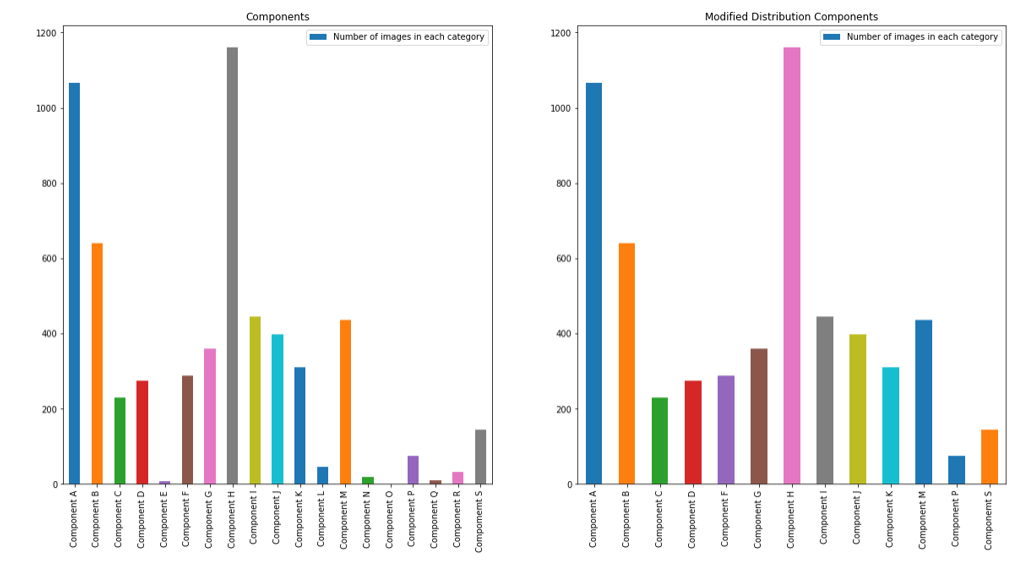
\includegraphics[width=.8\linewidth]{figures/03-Components.PNG}
  \caption{Components Labels}
  \label{fig:compolab}
\end{subfigure}
\caption[Pre processing of labels]{Label distributions before and after pre-processing. Some labels are cut out,  the order can be re-arranged in order to produce more powerful visualization}
\label{fig:labelsdistrib}
\end{figure}

\subsection{Data Augmentation}
%% Editing note: \url{http://www.sepmstrata.org/microscopic_gallery_details.aspx?gid=224&pg=2&gcid=10} is where I took pictures from. 
The networks used for this thesis are trained on data set of around 10,000,000 images. Our data set has 1907 images, this difference makes it likely that we will not have enough sample for our network to learn properly. A way for us to get more training data is to use data augmentation.  There is a  large number of techniques that can be used. As mentioned in Section \ref{sec:dataug}, the most common are rotations, flips, resizing, rescaling, cropping and adding of noise. But some of them can not be used in our case. 

Cropping is a great way to create multiple images from one image. But there is a risk to crop an irrelevant zone of the image. When classifying Components for example, on Figure~\ref{fig:crops}, we can see what could go wrong when cropping. Indeed, both images generated from the green and the yellow crops will have the same labels. The organism in the yellow crop is one of the components of the thin section, it will thus be one of the labels of the image. This means that both images will have this component as label, but it is not present in the second image. So we will teach our model the wrong information. A way of dealing with this would be to make big crops, so we keep most of the valuable information in each cropped image.  

\begin{figure}[h]
    \centering
        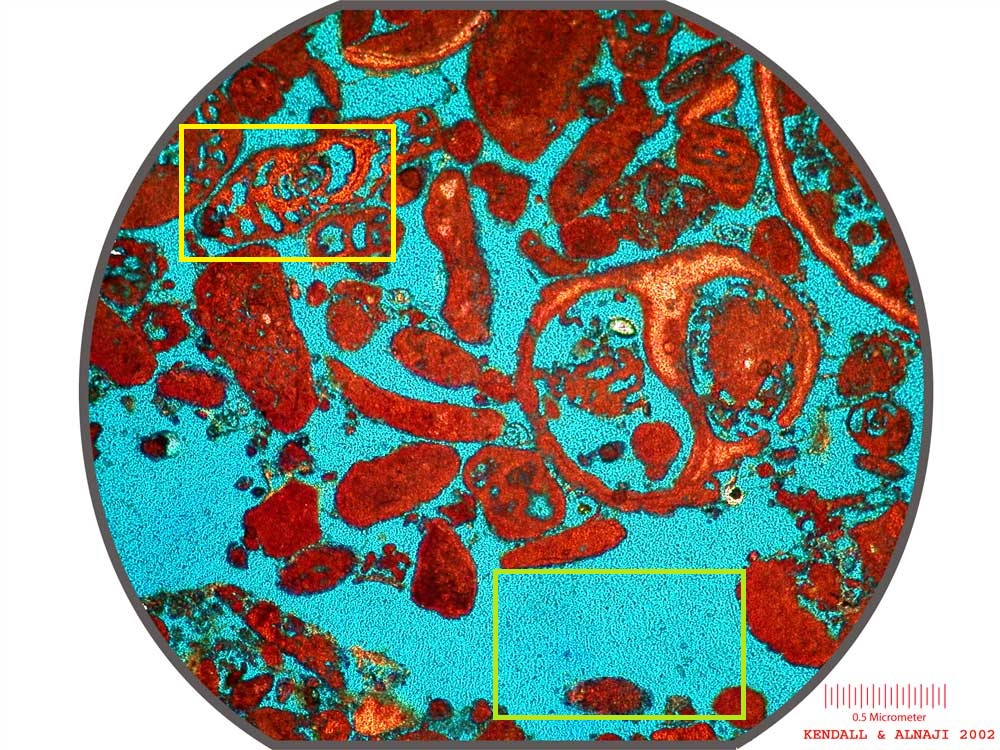
\includegraphics[width=0.3\textwidth]{figures/03-cropping_example_with2crops}
        \caption[Thin section with 2 random crops]{ Thin section with two random crops. The yellow and green crops have the same labels but contains very different information. This image has been adapted from \cite{section} which has a gallery of thin sections of carbonate rocks. }
        \label{fig:crops}
\end{figure}

When coring, a blue resin is injected into the core in order to keep fragments together. It also allows to see pores more clearly. It is thus important to maintain this blue color when doing data augmentation. That is why we can not change the colors in our images, techniques such as grayscale are discarded.


The augmentations used in this thesis are :
\begin{itemize}
    \item Color Jitter: In section \ref{sec:dataug}, we explained the way color jitter works. Now on Figures~\ref{fig:brightness} to ~\ref{fig:hue}, one can see how each parameters influence the image.
    We chose to keep all the parameters to 0.20. Except for hue that was kept to 0 since it is important to keep the colors unchanged. These values should remain small because we do not want to alter the image too much. If we do so, when we present it with new images, it will not be able to recognize them. 

\begin{figure}
\begin{subfigure}{.5\textwidth}
  \centering
  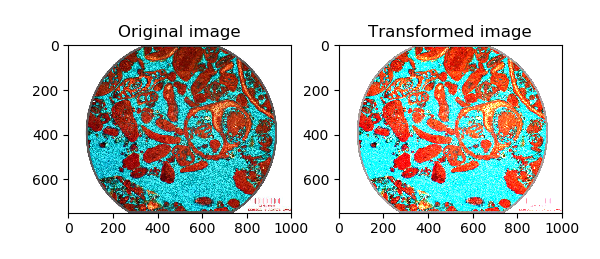
\includegraphics[width=.8\linewidth]{figures/03-bightness08.PNG}
  \caption{Brightness= 0.2}
  \label{fig:brightness}
\end{subfigure}%
\begin{subfigure}{.5\textwidth}
  \centering
  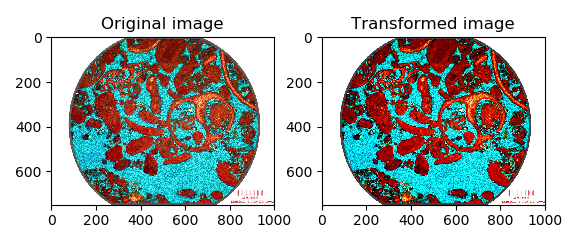
\includegraphics[width=.8\linewidth]{figures/03-contrast1.PNG}
  \caption{Contrast = 0.2}
  \label{fig:contrast}
\end{subfigure}
\begin{subfigure}{.5\textwidth}
  \centering
  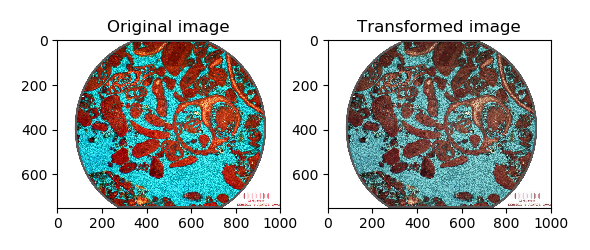
\includegraphics[width=.8\linewidth]{figures/03-saturation0.PNG}
  \caption{Saturation = 0.2}
  \label{fig:saturation}
\end{subfigure}%
\begin{subfigure}{.5\textwidth}
  \centering
  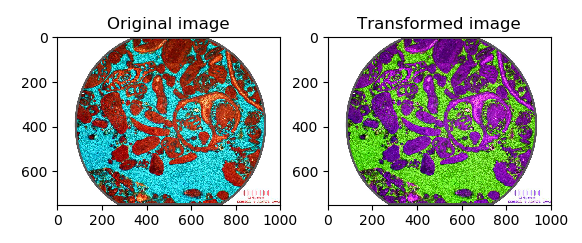
\includegraphics[width=.8\linewidth]{figures/03-hue05.PNG}
  \caption{Hue = 0.5}
  \label{fig:hue}
\end{subfigure}
\caption[Color Jitter Augmentation]{Images before and after being augmented with color jitter. The parameter indicated under the image is the only one that is not set to 0. It shows the impact of different the parameters of ColorJitter. The images have been adapted from a thin section collected at \cite{section}}
\label{fig:colorjitter}
\end{figure}

    \item Rotation: This was the first data augmentation technique we used. The images in our data set are thin sections pictures of core. The core that is drilled out is a cylinder, so the pictures are round. In order to focus on the relevant pixels, all the pixels outside of the circle have been put to 0. This also allowed to be able to rotate the image as much as we want. The way we actually proceed is that we draw a number between 0 and 360. This number is the angle at which we rotate the picture. So it combines every kind of rotation, flips.. that could be done. On Figure~\ref{fig:rotate}, we see how the rotation combined with a circle crop look.
\begin{figure}
\begin{subfigure}{.5\textwidth}
  \centering
  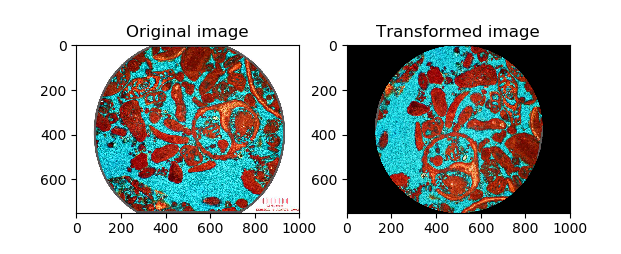
\includegraphics[width=.8\linewidth]{figures/03-rotation_260}
  \caption{Circle crop and 260 degrees rotation}
  \label{fig:rotate}
\end{subfigure}%
\begin{subfigure}{.5\textwidth}
  \centering
  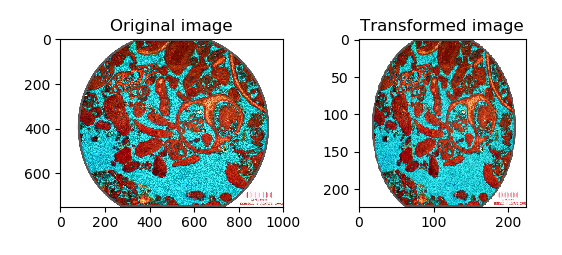
\includegraphics[width=.8\linewidth]{figures/03-resize.PNG}
  \caption{Resizing to 224x224 pixels}
  \label{fig:resize}
\end{subfigure}
\begin{subfigure}{.5\textwidth}
  \centering
  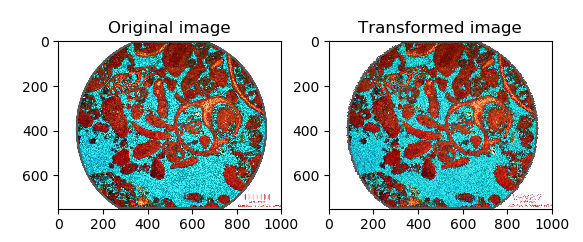
\includegraphics[width=.8\linewidth]{figures/03-elastic_trans_08_03.PNG}
  \caption{Elastic Transform with (\(\alpha\)=3, \(\sigma\)=0.3)}
  \label{fig:elastics1}
\end{subfigure}%
\begin{subfigure}{.5\textwidth}
  \centering
  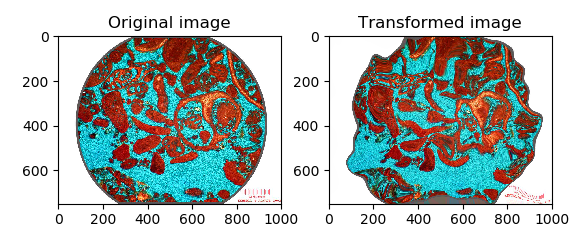
\includegraphics[width=.8\linewidth]{figures/03-elastic_trans_3000_30.PNG}
  \caption{Elastic Transform with (\(\alpha\)=3000, \(\sigma\)=30)}
  \label{fig:elastics2}
\end{subfigure}
\begin{subfigure}{.5\textwidth}
  \centering
  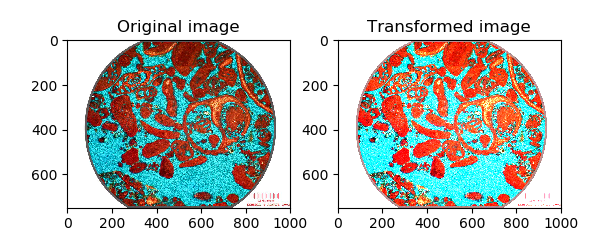
\includegraphics[width=.8\linewidth]{figures/03-medianscale}
  \caption{Median Scale}
  \label{fig:median}
\end{subfigure}
\caption[Various data augmentation]{Images before and after being augmented with various Data Augmentations. We perform all of them on the original sized image to make it more visible. But in practice we perform the resizing first, to optimize our computation time. These images have been adapted from a thin section collected at \cite{section}}
\label{fig:transfos}
\end{figure}

    \item Resizing: The pictures were initially 5000x5000 pixels. We resized them to sizes usable by different models (224x224 for ResNet18, 299x299 for Inception\_v3). This implies a loss in image quality but it drastically increases the speed of computation. See Figure~\ref{fig:resize}
    \item Elastic Transform : On Figure~\ref{fig:elastics1} and~\ref{fig:elastics2} , we have examples of two different sets of coefficients. The elastic transform on the first images looks more like adding some noise to the picture while the one on the right is extremely distorted. In our case, we can not use the second set of coefficients since we don't want to deform components so much that they are not identifiable anymore. 

    \item Median Scale : This scales with the median and the mean of each channel (red, green and blue) of the numpy array. This gives a more clear view of the picture as shown on Figure~\ref{fig:median}  
 \end{itemize}

After Data Augmentation, we have a dataset of 19070 images. 


\section{Experiments}
\subsection{Inception\_v3}
We use the Inception\_v3 version of the GoogLeNet. It is the latest version implemented and available on PyTorch, this is why we chose this version. The network is 22 layers deep, 27 if we count the pooling layer. A detailed view of its architecture is shown in Figure \ref{fig:googarch}.
We repeat 2D convolutions paired with batch normalization with various kernel sizes. Before the final fully connected layer, we also have a pooling layer. The inception module is as described in section \ref{sec:gogl}. We display a part of it to show how the kernel size is changed.  
\subsection{ResNet}
%% Editing note : (research paperresnet or imagenet webpage
ResNet is the network that gives theoretically the best results \cite{resnetpaper}. There are different versions of this network with different depths: Resnet18, Resnet50, Resnet101 etc... But we must keep in mind that we have a small data set compared to what is usually used for those networks. After data augmentation, we have around 19000 images. It is still far from ImageNet, so we should be careful about over-fitting. We can't use a too deep network on a small amount of data. That is why we chose to only use Resnet18. The architecture is presented on Figure~\ref{fig:resarchi}

After a first convolution layer, we use a basic block as shown on figure~\ref{fig:resarchi} that we repeat until the last layer. In this last layer, out\_features is the number of classes the network should output. 
\subsection{AxelNet}
AxelNet is a smaller network, only eight layers deep, so the lack of training data is not so critical in this case. It is divided in two parts: five convolutional layers to do the feature extraction and three linear layers to do the classification.  The details of the architecture are shown on Figure~\ref{fig:resarchi}
\begin{figure}
\begin{subfigure}{.5\textwidth}
  \centering
  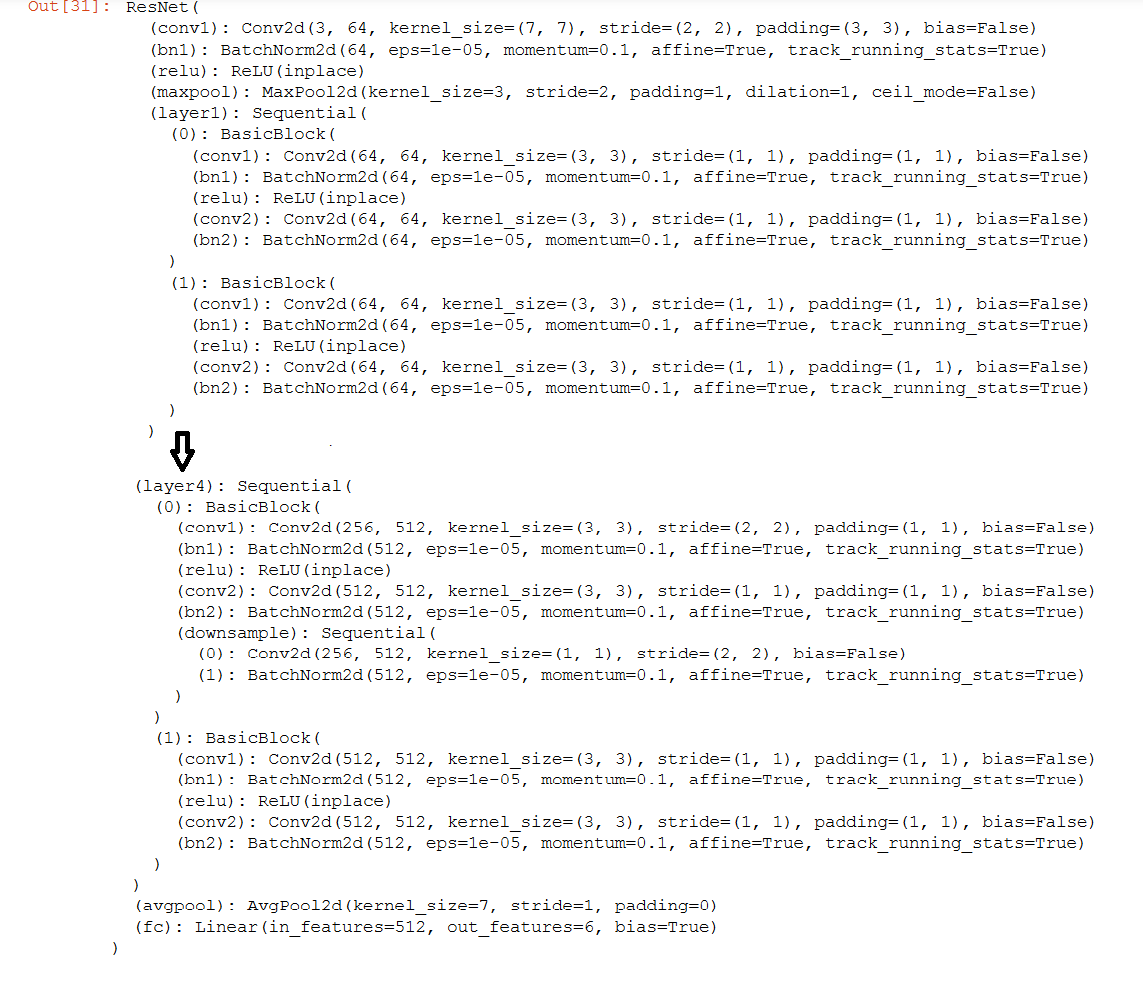
\includegraphics[width=6cm, height=3cm]{figures/03-Resnet_architecture}
  \caption{ResNet18}
  \label{fig:resarchi}
\end{subfigure}%
\begin{subfigure}{.5\textwidth}
  \centering
  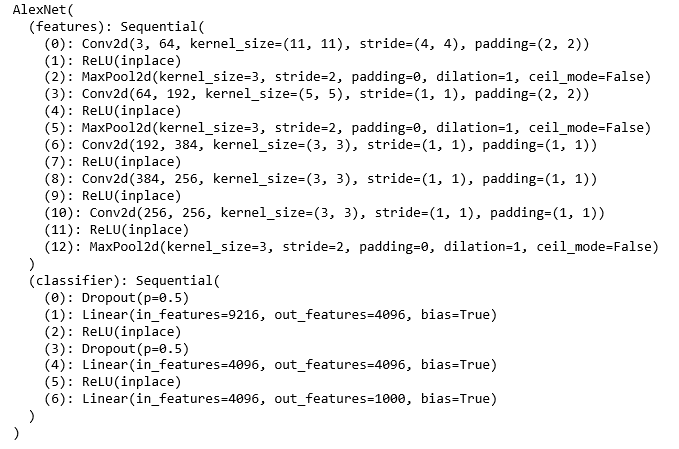
\includegraphics[width=6cm, height=3cm]{figures/03-alexnet_architecture}
  \caption{AlexNet}
  \label{fig:alexarchi}
\end{subfigure}
\begin{subfigure}{.5\textwidth}
  \centering
  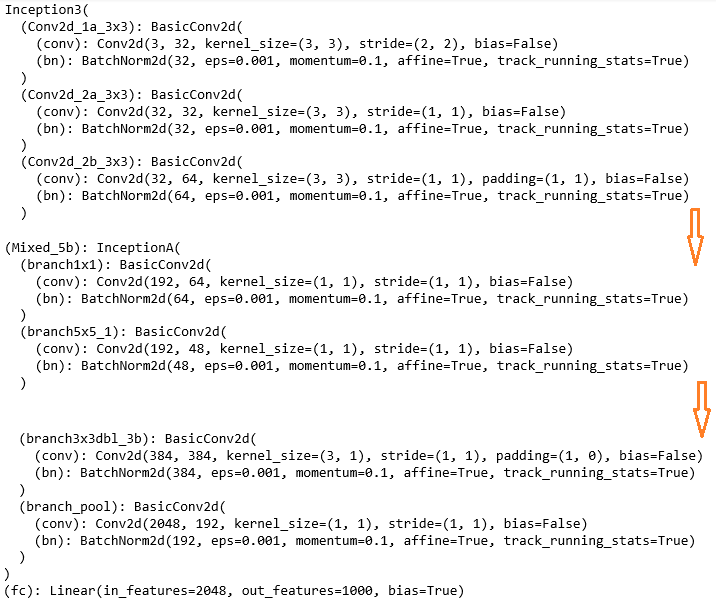
\includegraphics[width=6cm, height=3cm]{figures/03-inception_architecture}
  \caption{Inception\_v3}
  \label{fig:googarch}
\end{subfigure}
\caption[Networks architectures]{The architectures of the three networks. AlexNet is a simple eight layers network divided in two parts: feature extraction and classification. Resnet 18 is a deep network with a basic block repeated several times and a single linear layer in the end. Inception\_v3 is a 22 deep CNN with repeated Inception blocks.}
\end{figure}

\subsection{Hyper parameters}
Hyper parameters are the parameters that are chosen before training, and that will remain the same during the whole training. One of the questions in this thesis is to study the influence of some hyper parameters on the  convergence of the algorithm. To do so, we will make some of them may vary from one experiment to an other. 


\subsubsection{Weights initialization} \label{sec:init}
As mention in Section \ref{sec:translearn}, there are two ways of using the networks to perform a classification task. Either you train all the layers in the network and randomly initialize the weights. Or we use the weights that have achieved good results on known data set and retrain only a smaller part of the network to make it specific to the task.
Choosing between those two tasks depends on the size of the network and the size of the data set. If the network is too deep, training all the layers might lead to over-fitting. But if the data set is very big, then we need to train the whole model to make it recognize forms in our data set. 
We will conduct two trainings in parallel for each class. One with random initialization and one with pretraiend weights. 
When conducting those experiments, we use the Adam optimizer since we want to converge quickly to a minimum to compare the two approaches. 

After this first experiment, we will determine which networks performs best. We will also test the hypothesis that every class performs similarly with one specific network. So for example, if ResNet 18 performs better with pretrained weights on the Dunham class, it will do so also on the porosity class. This way we do not need to optimize our network on every one of the 4 classes. 

\subsubsection{Batch size}
The batch sized is fixed to 700 so that two experiments can be run in parallel on the same GPU for ResNet 18 and AlexNet. For Inception\_v3, the batch size is set to 50 to be able to run two experiments in parallel. In case we need to run more than two experiments in parallel, we reduce the batch size accordingly.

\subsubsection{Optimizers}
For Adamax, there is a set of default values for the hyper-parameters: \(\eta = 0.002\), \(\beta_1 = 0.9\) \(\beta_2 = 0.999\), \(\epsilon = 1e-8\) that we will keep across all experiments. We kept those from the default configuration of the optimizer. 
For the SGD, we choose an initial value of learning rate in [0.1, 0.01, 0.001] and implemented a learning rate decay every 30 iterations, and a momentum of 0.9. 

Adamax is used to get a good convergence quickly, this is why we use Adamax in the first experiment on the weight initialization. This first experiment is going to give us insight on which network performs best on the different labels. Then in a second experiment, we will try to optimize further the best performing model. To reach the best possible results We will use the SGD+momentum optimizer. We can then check the influence of the optimizer on our results. 

\subsubsection{Regularization}
As we mentioned before, the small amount of data we have make overfitting likely. In order to avoid this problem, we add a layer of dropout with probability 0.5 in AlexNet. Inception\_v3. ResNet and Inception\_v3 already performs batch normalization between every convolutional. That is a efficient way of doing regularization. This is why we did not add any dropout layer.  